

\documentclass{article}
\usepackage[utf8]{inputenc}
\usepackage{amsmath}
\usepackage{graphicx}

\title{Reporte de actividades semestre Septiembre 2020 a Marzo 2021}
\author{Julio César Pérez Pedraza}
\date{Marzo de 2021}

\begin{document}

\maketitle

\section{Introducción}
En el primer semestre, como se expuso en la reunión de comité tutorial, principalmente se realizaron avances en el estudio del método de Lattice Boltzmann clásico (LBM), para lo cual fue también necesario el aprendizaje del lenguaje de programación C. Además, se continuó con el estudio teórico de grafeno pristino y bajo deformaciones. Continuando con el plan de trabajo que hemos establecido, el semestre que apenas terminó se dedicó al estudio del método de Lattice Boltzmann relativista (RLBM), además de implementaciones de ejemplos básicos del caso clásico como lo son el flujo de Poiseuille con el propósito de adquirir práctica y experiencia en estas simulaciones. Al final del semestre, además, se comenzó con la implementación de un código relativista con el fin de primero aplicarlo a cálculos conocidos y posteriormente al sistema de interés en nuestro trabajo.\\

A continuación se da un breve resumen del trabajo desarrollado en este semestre. Se comienza con la teoría del RLBM, donde se obtienen expresiones para la ecuación de Lattice Boltzmann, funciones en equilibrio, operador de colisión y viscosidad cortante del sistema. Enseguida, se da un breve repaso al problema del flujo de Poiseuille en el caso clásico 2D, incluyendo el código que reproduce su comportamiento.

\section{Método de lattice Boltzmann relativista}
Basado en trabajos de Mendoza \textit{et al.}\footnote{M. Mendoza, B. M. Boghosian, H. J. Herrmann, and S. Succi, \textit{Derivation of the lattice Boltzmann Model for relativistic hydrodynamics}, Phys. Rev D \textbf{82}, 105008 (2010).}, el RLBM se basa en dos simples observaciones: (1) el formalismo cinético es naturalmente covariante/hiperbólico, y (2) basandonos en una representación discreta de la función de distribución cinética, con velocidad finita, el método de lattice Boltzmann estándar naturalmente tiene el aspecto de ecuaciones de estado de tipo relativistas, donde la velocidad del sonido, $c_s$ es una fracción de la velocidad de la luz $c$ y es la máxima velocidad de transporte de masa. Además, se escoge la velocidad de red cercana a la velocidad de la luz $c_l=\delta x / \delta t \sim c$ (a diferencia de aplicaciones de LBM estándares).\\

Consideramos las ecuaciones de fluidos relativistas asociadas con la conservación del número de partículas y energía-momento. El tensor de energía-momento se escribe como\footnote{ C. Cercignani and G. M. Kremer, \textit{The Relativistic Boltzmann Equation: Theory and Applications}, Birkhauser, Boston, 2002.} \footnote{R. Baier, P. Romatschke, D. T. Son, A.O. Starinets, and M. A. Stephanov, J. High Energy Phys.04 (2008) 100.}:
\begin{equation}
    T^{\mu\nu} = P \eta^{\mu\nu} + (\epsilon + P) u^\mu u^\nu+ \pi^{\mu\nu},
\end{equation}
donde $\epsilon$ es la densidad de energía, $P$ la presión hidrostática, y $\pi^{\mu\nu}$ la componente disipativa del tensor de energía-momento a especificarse mas tarde. Además, se define el cuadri-vector de velocidad (cuadri-velocidad) como 
\begin{equation}
    u^\mu = ( \gamma, \gamma \vec{\beta}),
\end{equation}
donde $\vec{\beta}= \vec{u}/c$ es la velocidad del fluido en unidades de la velocidad de la luz, y $\gamma =1/ \sqrt{1-|\vec{\beta}|^2}$ es el factor de Lorentz. También, el tensor $\eta^{\mu\nu}$ denota la métrica de Minkowski. Adicionalmente, se define el cuadri-vector de flujo de partículas (cuadri-flujo) como
\begin{equation}
    N^\mu = n \gamma (1, \vec{\beta})^\mu, 
\end{equation}
con $n$ el número de partículas por unidad de volumen. De estas definiciones, se puede aplicar la condición de conservación de energía-momento, $\partial_\mu T^{\mu\nu} =0$, obteniendo
\begin{subequations}
\begin{equation}
    \partial_t ((\epsilon +P)\gamma^2 -P) +\partial_a ((\epsilon+P)\gamma^2 u_a) + \partial_t \pi^{00} + \partial_a \pi^{a0} =0,
\end{equation}
\begin{equation}
   \partial_t ((\epsilon +P)\gamma^2 u_b) +\partial_b P +\partial_a ((\epsilon+P)\gamma^2 u_a u_b) + \partial_t \pi^{0b} + \partial_a \pi^{ab} =0,
\end{equation}
\end{subequations}
y la condición de conservación del número de partículas, $\partial_\mu N^\mu =0$, llegando a 
\begin{equation}
    \partial_t(n\gamma) + \partial_a (n\gamma u_a)=0.
\end{equation}
Se debe notar que, a diferencia del caso de fluidos no-relativistas, tenemos dos ecuaciones escalares, una para la energía y otra para el número de partículas. Para completar el set de ecuaciones es necesario especificar una ecuación de estado que relacione a al menos dos de las tres cantidades $n$, $P$ y $\epsilon$.

\subsection{Ecuación de Boltzmann relativista}
Las ecuaciones hidrodinámicas de arriba pueden ser derivadas como el límite macroscópico de la ecuación de Boltzmann relativista. Para el caso de un único gas no-degenerado y en la ausencia de fuerzas externas esta se escribe como$^2$
\begin{equation}
    \partial_\mu (p^\mu f) = \int (f^{'}_\star f^{'} - f_\star f) \Phi \sigma d\Omega \frac{d^3 p_\star}{p_{\star 0}},
\end{equation}
donde $p^\mu = \left( \frac{E(p)}{c}, \vec{p} \right)$ es el cuadri-momento de la partícula, $E(p) = (p^2c^2 + m^2 c^4)^{1/2}$ la energía relativista, $\sigma$ la sección eficaz diferencial, $\Omega$ el ángulo sólido y $\Phi$ el flujo invariante de Lorentz dado por$^2$
\begin{equation}
    \Phi = \sqrt{(p^\mu_\star p_\mu)^2 - m^2c^4},
\end{equation}
siendo estos tres últimos la base del llamado cilindro de colisión. Además, $f_\star\equiv f(\vec{x}, \vec{p_\star}, t)$ y $f\equiv f(\vec{x}, \vec{p}, t)$ denotan distribuciones antes de la colisión, mientras que $f^{'}_\star\equiv f(\vec{x}, \vec{p}^{'}_\star, t)$ y $f^{'}\equiv f(\vec{x}, \vec{p}^{'}, t)$ son las resultantes después de la colisión. El lado derecho de la Eq. (6) corresponde al término de colisión de la ecuación de Boltzmann, que se encarga de fijar los valores de los coeficientes de transporte en las ecuaciones macroscópicas. Dado que para el caso clásico el operador de colisión mas usado es el BGK, Marle\footnote{C. Marle, C. R. Hebd, Seances Acad. Sci. \textbf{260}, 6539 (1965).} propuso el primer operador BGK relativista dado por
\begin{equation}
    \partial_\mu (p^\mu f) = \frac{m}{\tau_M} (f^{eq}-f),
\end{equation}
donde $f^{eq}$ es el equilibrio relativista local, $m$ la masa en reposo de la partícula, y $\tau_m$ representa el tiempo característico entre colisiones subsecuentes, que puede pensarse como un tiempo de relajación solo para un sistema de referencia en reposo local, donde el momento de las partículas es cero$^2$. Sin embargo, para un sistema de referencia inercial general, el tiempo de relajación $\hat{\tau}_M$ se puede escribir como
\begin{equation}
    \hat{\tau}_M = \frac{p^0}{mc} \tau_M.
\end{equation}
Sin embargo, en el modelo de Marle los coeficientes de transporte no se pueden escribir en términos del tiempo de relajación $\hat{\tau}_M$ ya que depende de la componente $p_0$ del momento microscópico, y éste no puede aparecer en una descripción macroscópica. Para evitar ese problema, Takamoto y Inutsuka\footnote{M. Takamoto and S. Inatsuka, Physica A (Amstermdam).}, propusieron el modelo de Marle modificado, en el cual toman el tiempo de relajación como el promedio pesado $\frac{1}{\tau}= \langle \frac{1}{\hat{\tau}_M}\rangle$, de donde se obtiene la relación:
\begin{equation}
    \tau_M = \frac{K_1(\chi)}{K_2(\chi)}\tau,
\end{equation}
donde $\chi= \frac{mc^2}{kT}$ y $K_n$ es el segundo tipo de funciones de Bessel modificadas. El término de corrección $\frac{K_1(\chi)}{K_2(\chi)}$ tiende a 1 a bajas temperaturas ($\chi\rightarrow \infty$), y a $\frac{\chi}{2}$ a altas temperaturas, por lo que produce una buena aproximación a bajas temperaturas. Existe otro modelo de BGK más general que produce una buena aproximación a altas y bajas temperaturas, pero por el momento tomaremos el modelo de Marle modificado.

\subsection{Modelo de lattice Boltzmann relativista}
Al igual que en el caso clásico, se toma un set de velocidades discretas en cada punto de la red de acuerdo a las dimensiones de esta. En este documento describimos el método relativista de lattice Boltzmann para el caso de 3 dimensiones con el set de velocidades D3Q19, donde la velocidad máxima de movimiento de las partículas es $\sqrt{2}c_l$, con $c_l = \frac{\delta x}{\delta t}$, y en donde las unidades de velocidad son reescaladas de modo que $c\sim 1$. Como ya se había mencionado, la hidrodinámica relativista consta de dos escalares, densidad de energís y de número de partículas, por lo que es conveniente introducir dos funciones de distribución $f_i$ y $gi$ representando "fonones" y "fluones" respectivamente.\\

Las variables hidrodinámicas se calcula usando las siguientes restricciones macroscópicas
\begin{subequations}
\begin{equation}
    n\gamma = \sum_{i=0}^{18} f_i, 
\end{equation}
\begin{equation}
    (\epsilon+P) \gamma^2-P = \sum_{i=0}^{18} g_i, 
\end{equation}
\begin{equation}
    (\epsilon+P) \gamma^2 \vec{u} = \sum_{i=0}^{18} g_i \vec{c}_i. 
\end{equation}
\end{subequations}
Se tienen cinco ecuaciones y seis incógnitas ($n$, $\epsilon$, $P$ y $\vec{u}$), por lo que se ciera el sistema escogiendo una ecuación de estado, que este caso tomamos como $\epsilon= 3P$ (aunque puede tomarse cualquier otra).\\

Para obtener las ecuaciones de Boltzmann relativistas con el modelo de Marle a bajas temperaturas (modificado) comenzamos escribiendo explícitamente la Ec. (8) como
\begin{equation}
    \partial_0 (p^0 f) + \partial_a ( p^mu f) = \frac{m}{\tau_M} (f^{eq} -f).
\end{equation}
Usando el hecho de que las coordenadas espaciales y de velocidad son linealmente independientes, y reemplazando la Ec. (9), se puede llevar la Ec. (12) a la forma
\begin{equation}
    \partial_0 f + c^a \partial_a f = \frac{1}{\hat{\tau}_M} (f^{eq} -f),    
\end{equation}
donde $c^a$ son las velocidades microscópicas. De acuerdo al modelo de Marle modificado$^5$, la Ec. (13) se puede escribir como
\begin{equation}
    \partial_0 f + c^a \partial_a f = \left( \frac{1}{\tau}-\theta \right)  (f^{eq} -f),
\end{equation}
 donde el término de corrección $\theta$, usando la Ec. (10) está dado por
 \begin{equation}
     \theta = \left[ \left\langle \frac{1}{\tau_{M\star}} \right\rangle - \frac{1}{\tau_{M\star}} \right] = \frac{1}{\tau_M}\left[ \frac{K_1(\chi)}{K_2(\chi)}-\frac{1}{\gamma_v} \right],
 \end{equation}
donde $\gamma_v$ es el factor de Lorentz para las velocidades microscópicas. Para temperaturas bajas se tiene que $\frac{K_1(\chi)}{K_2(\chi)} \sim 1$ y $\gamma_v \sim 1$, por lo que la correción tiende a cero, recobrando la ecuación de Boltzmann no-relativista. Además, para temperaturas altas la correción se puede aproximar por
\begin{equation}
    \theta \approx \frac{\chi}{2} \frac{1}{\tau_M},
\end{equation}
que también tiende a desvanecerse conforme la temperatura se hace más grande. Por lo tanto, se recupera en ambos casos, bajas temperaturas y altas temperaturas, ecuaciones de Boltzmann clásicas para $f$ y $g$
\begin{equation}
    f_i(\vec{x} + \vec{c}_i\delta t, t + \delta t) -f_i (\vec{x}, t) = - \frac{\delta t}{\tau} (f_i - f_i^{eq}),
\end{equation}
y
\begin{equation}
    g_i(\vec{x} + \vec{c}_i\delta t, t + \delta t) -g_i (\vec{x}, t) = - \frac{\delta t}{\tau} (g_i - g_i^{eq}),
\end{equation}
con $\tau$ representando el tiempo de relajación realista del sistema.\\
    
Para calcular las funciones de distribución de equilibrio que recuperan las ecuaciones de fluidos relativistas, Ecs. (4) y (5), se usa el procedimiento de moment-matching entre las funciones de equilibrio y reglas de conservación, fijando así los parámetros de Lagrange. Explícitamente, se escriben las funciones de distribución de equilibrio como
\begin{subequations}
\begin{equation}
    f_i^{eq} = w_i [A + \vec{c}_i \cdot \vec{B}], \ \ for \ \ i\geq 0, 
\end{equation}
\begin{equation}
    g_i^{eq} = w_i [C + \vec{c}_i \cdot \vec{D} + E:(\vec{c}_i \vec{c}_i -\alpha I], \ \ for \ \ i > 0, 
\end{equation}
\begin{equation}
g_0^{eq} = w_0 [F], 
\end{equation}
 \end{subequations}
 donde $\alpha$, $A$, $\vec{B}$, $C$, $\vec{D}$, $\overleftrightarrow{E}$ y $F$ son parámetroa de Lagrange a fijarse de acuerdo a las constricciones macroscópicas de conservación. Usando los pesos definidos por $w_0=1/3$, $w_i=1/18$ para velocidades con magnitud $|\vec{c}_i|=c_l$ y $w_i = 1/36$ para velocidades con $|\vec{c}_i|=\sqrt{2}c_l$.\\
 
 Para encontrar $A$ y $\vec{B}$, se imponen las condiciones 
 \begin{equation}
     \sum_{1=0}^{18} f_i^{eq} = n\gamma,
 \end{equation}
 y
 \begin{equation}
     \sum_{1=0}^{18} f_i^{eq} \vec{c}_i = n\gamma\vec{u},
 \end{equation}
 emcontrando los valores $A=n\gamma$ y $\vec{B}= \frac{
 3}{c_l^2}\gamma n \vec{u}$. Después, se debe obtener la Ec. (4) de las funciones de equilibrio $g_i^{eq}$, por lo que se toman las siguientes restricciones
 \begin{equation}
     \sum_{1=0}^{18} g_i^{eq} = \gamma^2 (\epsilon +P) -P,
 \end{equation}
 \begin{equation}
     \sum_{1=0}^{18} g_i^{eq} \vec{c}_i = (\epsilon+P)\gamma^2\vec{u},
 \end{equation}
 y adicionalmente
 \begin{equation}
     \sum_{1=0}^{18} g_i^{eq} c_{ia}c_{ib} = P \delta_{ab} +(\epsilon+P) \gamma^2 u_a u_b.
 \end{equation}
 Se encuentran las expresiones para los parámetros de Lagrange $\alpha= \frac{c_l^2}{3}$, $C=\frac{3P}{c_l^2}$, $\vec{D}= \frac{3}{c_l^2}(\epsilon+P) \gamma^2 \vec{u}$, $E_{ab}=\frac{9}{2c_l^4}(\epsilon+P) \gamma^2 u_a u_b$ y $F= (\epsilon+P) \gamma^2\left[ 3- 3\frac{(2+c_l^2)P}{c_l^2(\epsilon+P)\gamma^2}- \frac{3}{2c_l^2} (\epsilon+P)\gamma^2|\vec{u}|^2 \right].$ Por lo tanto, se llega a las funciones de distribución de equilibrio que recuperan las ecuaciones de fluidos relativistas en el límite continuo dadas por
  \begin{equation}
     f_i^{eq} = w_i n\gamma\left[ 1+3 \frac{(\vec{c}_i\cdot \vec{u})}{c_l^2} \right], 
 \end{equation}
 para $i\geq 0$, 
 \begin{equation}
     g_i^{eq} = w_i(\epsilon+P)\gamma^2\left[ \frac{3P}{c_l^2(\epsilon+P)\gamma^2}+3 \frac{(\vec{c}_i\cdot \vec{u})}{c_l^2}+ \frac{9}{2} \frac{(\vec{c}_i\cdot \vec{u})^2}{c_l^4}-\frac{3}{2}\frac{|\vec{u}|^2}{c_l^2} \right], 
 \end{equation}
  para $i> 0$, y
   \begin{equation}
     g_0^{eq} = w_0(\epsilon+P)\gamma^2\left[3- \frac{3P(2+c_l^2)}{c_l^2(\epsilon+P)\gamma^2}-\frac{3}{2}\frac{|\vec{u}|^2}{c_l^2} \right], 
 \end{equation}
 para partículas en reposo. Además, mediante la elección de la ecuación de estado $\epsilon=3P$, estas ecuaciones se simplifican a 
   \begin{equation}
     f_i^{eq} = w_i n\gamma\left[ 1+3 \frac{(\vec{c}_i\cdot \vec{u})}{c_l^2} \right], 
 \end{equation}
 para $i\geq 0$, 
 \begin{equation}
     g_i^{eq} = w_i\epsilon\gamma^2\left[ \frac{1}{c_l^2\gamma^2}+4 \frac{(\vec{c}_i\cdot \vec{u})}{c_l^2}+ 6 \frac{(\vec{c}_i\cdot \vec{u})^2}{c_l^4}-2\frac{|\vec{u}|^2}{c_l^2} \right], 
 \end{equation}
  para $i> 0$, y
   \begin{equation}
     g_0^{eq} = w_0\epsilon\gamma^2\left[4- \frac{2+c_l^2}{c_l^2\gamma^2}-2\frac{|\vec{u}|^2}{c_l^2} \right], 
 \end{equation}
 para $i=0$. La viscosidad cortante se calcula como $\eta = \frac{4}{9} \gamma \epsilon (\tau-\delta t /2) c_l^2$. Además, es importante notar que este esquema relativista recupera suavemente el límite no-relativista simplemente haciendo $\beta \rightarrow 0$.
 
\section{Flujo clásico de Poiseuille}

El flujo de Poiseuille es uno de los casos mas representativos y utilizados en LBM ya que dado a que contiene solución analítica es muy útil para comparar los resultados analíticos con los resultados numéricos.\\

El flujo de Poiseuille consiste en el flujo de fluido incompresible y estable atrapado entre dos paredes paralelas separadas una distancia $d$ sobre el eje $y$. El flujo puede ser resultado de ya sea (i) un gradiente de presión constante o (ii) una fuerza externa tal como la gravedad en la dirección $x$. Además se asume la condición de no-slip entre el fluido y las paredes.\\

En el caso en el cual el flujo es debido a un gradiente de presión, el perfil de velocidad analítico está dado por
\begin{equation}
    u_x(y)= -\frac{1}{2\eta} \frac{dp}{dx} (y-y_{bot})(y-y_{top}),
\end{equation}
representanto esto una solución con perfil parabólico sobre la dirección $x$.\\

\subsection{Código en C}
En el siguiente programa que simula el flujo de Poiseuille en 2D, se utilizó el esquema D2Q9 con un set discreto de 9 velocidades. Se utilizaron condiciones de frontera periódicas sobre el eje $x$ y condiciones de frontera fullway bounce back (BB) considerando la frontera en medio de los nodos frontera y sólidos del sistema. Las condiciones de frontera inlet y outlet sobre la dirección $x$ están dadas por $\rho_{out} = 1$ (en unidades de simulación), $\rho_{in}= \rho_{out} + \Delta p$, con $\Delta p=\frac{8\eta u_c}{(y_{top}-y_{bot})^2} (x_{out} - x_{in})$, donde $u_c=0.1$ es la velocidad máxima a la que pueden viajar las partículas. Con estas condiciones la solución analítica está dada por
\begin{equation}
     u_x(y)= -\frac{1}{2\eta} \frac{\Delta p}{(x_{out} - x_{in})} (y-y_{bot})(y-y_{top}).
\end{equation}\\

A continuación se muestra el código implementado para este problema. La Fig. 1 muestra el perfil obtenido numéricamente, el cual tiene la forma que se espera de la solución analítica.

\begin{figure}[h]
\centering
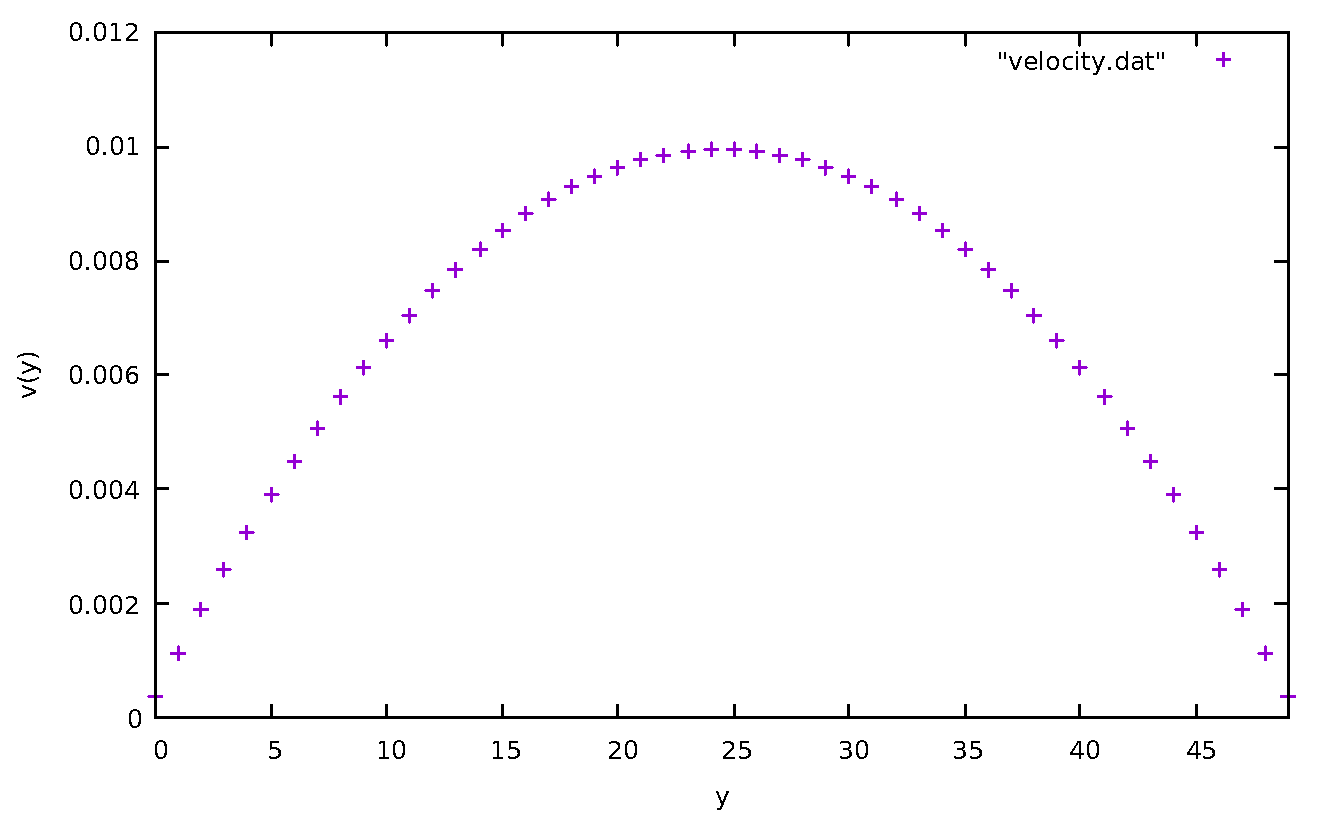
\includegraphics[scale=0.58]{Poiseuille.pdf}
\caption{Perfil de velocidad en dirección $x$ del flujo de Poiseuille 2D}
\end{figure}

\end{document}
